\documentclass[tikz,border=12pt]{standalone}
\usepackage{amsmath,amssymb}
\usepackage{tikz}
\usetikzlibrary{arrows.meta}

\begin{document}
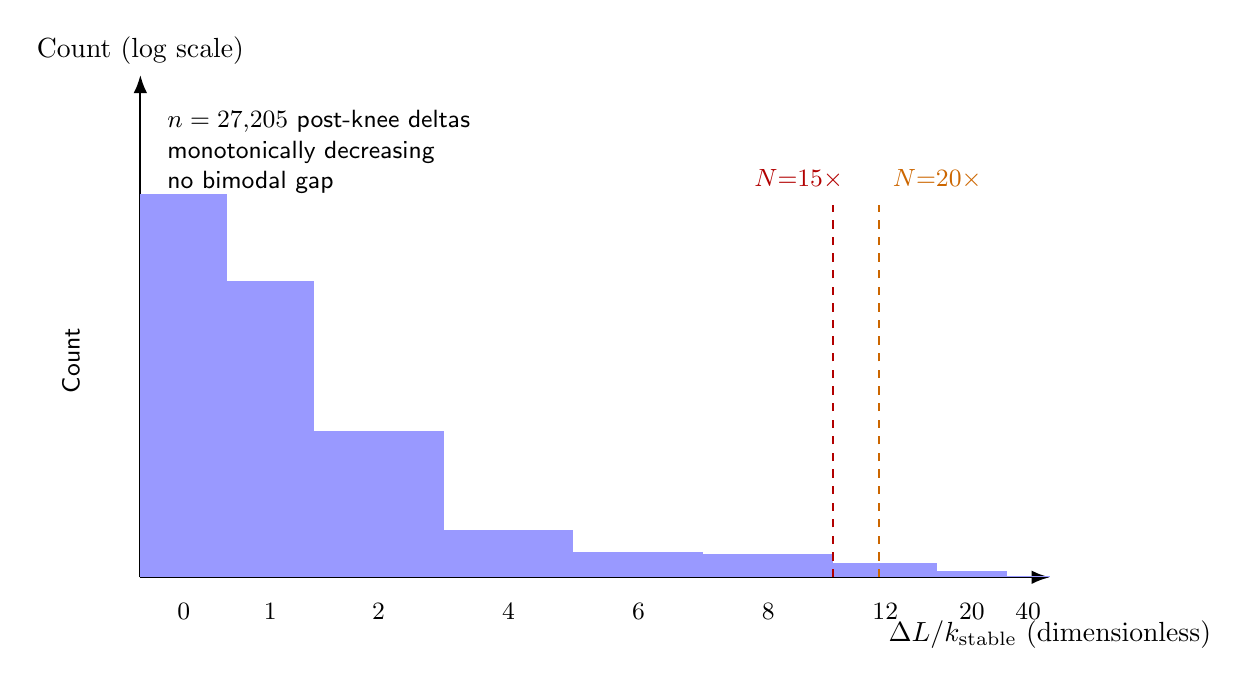
\begin{tikzpicture}[
  scale=1.1,
  >=Latex,
  annot/.style={font=\small\sffamily,align=left},
]

% Axes — leave bottom margin for labels
\draw[->,thick] (0,0) -- (10.5,0) node[below=12pt] {$\Delta L / k_{\text{stable}}$ (dimensionless)};
\draw[->,thick] (0,0) -- (0,5.8) node[above] {Count (log scale)};

% Bars
\fill[blue!40] (0.0,0) rectangle (1.0,4.43);
\fill[blue!40] (1.0,0) rectangle (2.0,3.42);
\fill[blue!40] (2.0,0) rectangle (3.5,1.69);
\fill[blue!40] (3.5,0) rectangle (5.0,0.54);
\fill[blue!40] (5.0,0) rectangle (6.5,0.29);
\fill[blue!40] (6.5,0) rectangle (8.0,0.27);
\fill[blue!40] (8.0,0) rectangle (9.2,0.16);
\fill[blue!40] (9.2,0) rectangle (10.0,0.07);
\fill[blue!40] (10.0,0) rectangle (10.5,0.01);

% Bin edge labels — more breathing room below x-axis
\node[annot,below=6pt] at (0.5,0)  {$0$};
\node[annot,below=6pt] at (1.5,0)  {$1$};
\node[annot,below=6pt] at (2.75,0) {$2$};
\node[annot,below=6pt] at (4.25,0) {$4$};
\node[annot,below=6pt] at (5.75,0) {$6$};
\node[annot,below=6pt] at (7.25,0) {$8$};
\node[annot,below=6pt] at (8.6,0)  {$12$};
\node[annot,below=6pt] at (9.6,0)  {$20$};
\node[annot,below=6pt] at (10.25,0){$40$};

% Top-left annotation
\node[annot,anchor=north west] at (0.2,5.5) {$n = 27{,}205$ post-knee deltas\\monotonically decreasing\\no bimodal gap};

% Threshold lines — shorter, better spacing
\draw[red!70!black,thick,dashed] (8.0,0) -- (8.0,4.3);
\node[annot,red!70!black,anchor=south,inner sep=4pt] at (7.6,4.35)
  {$N{=}15{\times}$};

\draw[orange!80!black,thick,dashed] (8.53,0) -- (8.53,4.3);
\node[annot,orange!80!black,anchor=south,inner sep=4pt] at (9.2,4.35)
  {$N{=}20{\times}$};

% y-axis label
\node[annot] at (-0.8,2.5) {\rotatebox{90}{Count}};

\end{tikzpicture}
\end{document}
